% ŠABLONA PRO PSANÍ ZÁVĚREČNÉ STUDIJNÍ PRÁCE
%%%%%%%%%%%%%%%%%%%%%%%%%%%%%%%%%%%%%%%%%%%%
% Autor: Jakub Dokulil (kubadokulil99@gmail.com)
% Tato šablona byla vytvořena tak, aby pomocí ní mohli v systému LaTeX soutěžící sázet své práce a zároveň odpovídala požadavkům na formátování vyplývajícím z wordové šablony umístěné na webu soc.cz.
%
\documentclass[12pt, a4paper,
%oneside,      %% -- odkomentujte, pokud chcete svou práci mít pouze jednostrannou, mezera pro hřbet pak automaticky bude pouze na levé straně
twoside,        %% -- pro oboustranné práce, mezera pro hřbet následně střídá strany.
openright
]{report}

%% Nutné balíčky a nastavení
%%%%%%%%%%%%%%%%%%%%%%%%%%%%

%% Proměnné
\newcommand\obor{INFORMAČNÍ TECHNOLOGIE} %% -- napiš číslo a název tvého oboru
\newcommand\kodOboru{18-20-M/01} %% -- napiš číslo a název tvého oboru
\newcommand\zamereni{se zaměřením na počítačové sítě a programování} %% -- napiš číslo a název tvého oboru
\newcommand\skola{Střední škola průmyslová a umělecká, Opava} %% vyplň název školy
\newcommand\trida{IT4} %% vyplň jméno svého konzultanta
\newcommand\jmenoAutora{Michaela Říčná}  %% vyplň své jméno
\newcommand\skolniRok{2023/24} %% vyplň rok
\newcommand\datumOdevzdani{1. 1. 2024} %% vyplň rok
\newcommand\nazevPrace{Mobilní aplikace s rozšířenou realitou} %% vyplň název své práce


\title{\nazevPrace} %% -- Název tvé práce
\author{\jmenoAutora} %% -- tvé jméno
\date{\datumOdevzdani} %% -- rok

\usepackage[top=2.5cm, bottom=2.5cm, left=3.5cm, right=1.5cm]{geometry} %% nastaví okraje, left -- vnitřní okraj, right -- vnější okraj

\usepackage[czech]{babel} %% balík babel pro sazbu v češtině
\usepackage[utf8]{inputenc} %% balíky pro kódování textu
\usepackage[T1]{fontenc}
\usepackage{cmap} %% balíček zajišťující, že vytvořené PDF bude prohledávatelné a kopírovatelné

\usepackage{graphicx} %% balík pro vkládání obrázků

\usepackage{subcaption} %% balíček pro vkládání podobrázků
\usepackage{float}
\usepackage{hyperref} %% balíček, který v PDF vytváří odkazy

\linespread{1.25} %% řádkování
\setlength{\parskip}{0.5em} %% odsazení mezi odstavci


\usepackage[pagestyles]{titlesec} %% balíček pro úpravu stylu kapitol a sekcí
\titleformat{\chapter}[block]{\scshape\bfseries\LARGE}{\thechapter}{10pt}{\vspace{0pt}}[\vspace{-22pt}]
\titleformat{\section}[block]{\scshape\bfseries\Large}{\thesection}{10pt}{\vspace{0pt}}
\titleformat{\subsection}[block]{\bfseries\large}{\thesubsection}{10pt}{\vspace{0pt}}


\usepackage{tocloft} % Balíček umožní přizpůsobit vzhled tabulky obsahu
\setlength{\cftbeforechapskip}{0pt}  % Menší rozestup pro kapitoly
\setlength{\cftbeforesecskip}{0pt}   % Menší rozestup pro sekce

\setcounter{secnumdepth}{2}
\setcounter{tocdepth}{1}
\usepackage{fancyhdr}
\pagestyle{fancy}
\fancyhf{}
\renewcommand{\headrulewidth}{0pt}
\fancyfoot[C]{\thepage}



\usepackage{booktabs}

\usepackage{url}

%% Balíčky co se můžou hodit :) 
%%%%%%%%%%%%%%%%%%%%%%%%%%%%%%%

\usepackage{pdfpages} %% Balíček umožňující vkládat stránky z PDF souborů, 

\usepackage{upgreek} %% Balíček pro sazbu stojatých řeckých písmen, třeba u jednotky mikrometr. Například stojaté mí: \upmu, stojaté pí: \uppi

\usepackage{amsmath}    %% Balíčky amsmath a amsfonts 
\usepackage{amsfonts}   %% pro sazbu matematických symbolů
\usepackage{esint}     %% pro sazbu různých integrálů (např \oiint)
\usepackage{mathrsfs}
\usepackage{helvet} % Helvet font
\usepackage{mathptmx} % Times New Roman
\usepackage{Oswald} % Oswald font


%% makra pro sazbu matematiky
\newcommand{\dif}{\mathrm{d}} %% makro pro sazbu diferenciálu, místo toho
%% abych musel psát '\mathrm{d}' mi stačí napsat '\dif' což je mnohem 
%% kratší a mohu si tak usnadnit práci

\let\oldchapter\chapter
\renewcommand{\chapter}{
	\clearpage
	\pagestyle{fancy}
	\oldchapter
}

\usepackage{listings}
\usepackage{xcolor}

\renewcommand{\lstlistingname}{Kód}% Listing -> Algorithm
\renewcommand{\lstlistlistingname}{Seznam programových kódů}% List of Listings -> List of Algorithms


%copied code start
\definecolor{mediumgray}{rgb}{0.3, 0.4, 0.4}
\definecolor{mediumblue}{rgb}{0.0, 0.0, 0.8}
\definecolor{forestgreen}{rgb}{0.13, 0.55, 0.13}
\definecolor{darkviolet}{rgb}{0.58, 0.0, 0.83}
\definecolor{royalblue}{rgb}{0.25, 0.41, 0.88}
\definecolor{crimson}{rgb}{0.86, 0.8, 0.24}

\lstdefinestyle{csh}{
	language=C,
	backgroundcolor=\color{white},
	basicstyle=\ttfamily,
	breakatwhitespace=false,
	breaklines=false,
	captionpos=b,
	columns=fullflexible,
	commentstyle=\color{mediumgray}\upshape,
	emph={},
	emphstyle=\color{crimson},
	extendedchars=true,  % requires inputenc
	fontadjust=true,
	frame=single,
	identifierstyle=\color{black},
	keepspaces=true,
	keywordstyle=\color{mediumblue},
	keywordstyle={[2]\color{darkviolet}},
	keywordstyle={[3]\color{royalblue}},
	literate=%
	{á}{{\'a}}1 {č}{{\v{c}}}1 {ď}{{\v{d}}}1 {é}{{\'e}}1 {ě}{{\v{e}}}1
	{í}{{\'i}}1 {ň}{{\v{n}}}1 {ó}{{\'o}}1 {ř}{{\v{r}}}1 {š}{{\v{s}}}1
	{ť}{{\v{t}}}1 {ú}{{\'u}}1 {ů}{{\r{u}}}1 {ý}{{\'y}}1 {ž}{{\v{z}}}1,		
	numbers=left,
	numbersep=5pt,
	numberstyle=\tiny\color{black},
	rulecolor=\color{black},
	showlines=true,
	showspaces=false,
	showstringspaces=false,
	showtabs=false,
	stringstyle=\color{forestgreen},
	tabsize=2,
	title=\lstname,
	upquote=true  % requires textcomp	
}
% copied code end






%% Bordel pro práci - můžeš smáznout :) 
%%%%%%%%%%%%%%%%%%%

\usepackage{lipsum} %% balíček který píše lipsum (nesmyslný text, který se používá pro kontrolu typografie)

%% Začátek dokumentu
%%%%%%%%%%%%%%%%%%%%
\begin{document}
	
	\pagestyle{empty}
	\pagenumbering{Roman}
	
	\cleardoublepage

%% Titulní stránka s informacemi
%%%%%%%%%%%%%%%%%%%%%%%%%%%%%%%%%%%%%%%%
	
	{\fontfamily{phv}\selectfont
		%% Logo školy
		\begin{figure}[h]
			\centering
			
\includegraphics[width=0.6\linewidth]{image/logo-skoly.png} 
		\end{figure}
		
		
		%% Hlavička práce a její název (viz proměnná \nazev prace)
		%% \sffamily %%% bezpatkové písmo - sans serif
		{\bfseries %%% písmo na stránce je tučně
			\begin{center}
				\vspace{0.025 \textheight}
				\LARGE{ZÁVĚREČNÁ STUDIJNÍ PRÁCE}\\
				\large{dokumentace}\\
				\vspace{0.075 \textheight}
				\LARGE {\nazevPrace}\\
			\end{center}  
		}%%%
		
		\begin{figure}[h]
			\centering
			
\includegraphics[width=0.5\linewidth]{image/logo.png} 
		\end{figure}
		
		\vspace{0.02 \textheight}
		\begin{table}[h!]
			\begin{tabular}{ll}
				\textbf{Autor:} & \jmenoAutora\\ 
				\textbf{Obor:} & \kodOboru { } \obor\\
				\textbf{} & \zamereni\\
				\textbf{Třída:} & \trida\\
				\textbf{Školní rok:} & \skolniRok\\
			\end{tabular}
			
		\end{table}		
	}
	
\cleardoublepage %% Zalomení dvojstránky
	
%% Stránka obsahující poděkování 
%%%%%%%%%%%%%%%%%%%%%%%%%%%%%%%%%%%%%%%%%%%%%%%%%%%%%%%%

%% Poděkování - nepovinné
%%%%%%%%%%%%%%%%%%%%%%%%%%%%
	

	
	\vspace*{0.7\textheight} %% Vertikální mezeru je možné upravit

%% Prohlášení - povinné
%%%%%%%%%%%%%%%%%%%%%%%%%%%%
	\noindent{\large{\bfseries{Prohlášení}\\}}  %% uprav si koncovky podle toho na jaký rod se cítíš, vypadá to pak lépe :) 
	\noindent{Prohlašuji, že jsem závěrečnou práci vypracovala samostatně a uvedla veškeré použité 
		informační zdroje.\\}
	\noindent{Souhlasím, aby tato studijní práce byla použita k výukovým a prezentačním účelům na Střední průmyslové a umělecké škole v Opavě, Praskova 399/8.}
	\vfill
	\noindent{V Opavě \datumOdevzdani\\}
	\noindent
	\begin{minipage}{\linewidth}
		\hspace{9.5cm} 
		\begin{tabular}{@{}p{6cm}@{}}
			\dotfill \\
			Podpis autora
		\end{tabular}
	\end{minipage}
	
	\cleardoublepage %% Zalomení dvojstránky

%% Stránka obsahující abstrakt (anotaci)
%%%%%%%%%%%%%%%%%%%%%%%%%%%%%%%%%%%%%%%%%%%%%%%%%%%%%%%%	

%% Abstrakt v češtině
%%%%%%%%%%%%%%%%%%%%%%%%%%%%
	\noindent{\Large{\bfseries{Abstrakt}\\}}
Práce se zabývá tvorbou mobilní aplikace s rozšířenou realitou na základě obrázků. Součástí práce byla tvorba 3D objektů a vytvoření mobilní aplikace. Výsledkem práce je funkční mobilní aplikace, která byla vytvořená za pomoci Unity, ve které je možné interagovat s určitými 3D objekty, které se zobrazují podle obrázků. Aplikace má celkem pět obrázků, kde každý z~nich má alespoň jeden 3D objekt. Mezi tyto objekty patří interaktivní dáma, kreslení, počítač s~interaktivními komponenty, které při kliknutí zobrazí menu, ukázka čtyř součástek učebny mechatroniky, kde dvě z nich zahrnují i animaci pohybu součástky, a model domu z animovaného seriálu.  

	
	\vspace{18pt}
	
	\noindent{\large{\bfseries{Klíčová slova}}}
	
	\noindent Rozšířená realita, sledování obrázků, Unity, 3D objekty, mobilní aplikace
	
	\vspace{18pt}

%% Abstrakt v angličtině
%%%%%%%%%%%%%%%%%%%%%%%%%%%%	
	\noindent{\Large{\bfseries{Abstract}}}
	
This project deals with creation of an AR mobile application based on images. Part of the project was modelling 3D objects and creating a mobile application.  The result of this project is a functional mobile application made in Unity in which the user can interact with specific 3D objects that are displayed according to images. 
The application has a total of five images, each of which contains at least one 3D object. Among these objects are an interactive checkers game, drawing, a computer with interactive components that display a menu when clicked, a~demonstration of four components in a mechatronics classroom, where two of them include animation of the component's movement, and a model of a house from an animated series.
	
	\vspace{18pt}
	
	\noindent{\large{\bfseries{Keywords}}}
	
	\noindent Augmented Reality, image tracking, Unity, 3D objects, mobile application
	
	\cleardoublepage %% Zalomení stránky

%% Stránka s generovaným obsahem
%%%%%%%%%%%%%%%%%%%%%%%%%%%%%%%%%%%%%%%	
	
	\tableofcontents %% Vygeneruje tabulku s obsahem

	\pagenumbering{arabic} %% Nastavení způsobu číslování stránek (alternativy roman | Roman)
	\setcounter{page}{1} %% Nastavení počitadla stránek

%% Stránka s úvodem - povinná část
%%%%%%%%%%%%%%%%%%%%%%%%%%%%%%%%%%%%%%%		
	\chapter*{Úvod}
	\addcontentsline{toc}{chapter}{Úvod}
Cílem mé práce bylo vytvořit mobilní aplikaci s rozšířenou realitou.  Původně jsem zamýšlela vytvořit AR aplikaci na základě lokace.  Z tohoto nápadu jsem nakonec ustoupila po zjištění, že GPS v mobilních zařízeních není přesné a balíček pro Unity zabývající se touto problematikou nebyl ke stažení zdarma, proto jsem se rozhodla vytvořit aplikaci na základě obrázků.
 
Hlavní motivací bylo pochopit základy rozšířené reality a Unity. Také jsem si přála pracovat na projektu, pro který bych si mohla vytvořit své vlastní 3D modely, jelikož mě modelování minulý rok zaujalo.  

Tato práce nejprve popisuje problematiku rozšířené reality. Poté se zaměřuje na tvorbu 3D objektů s ukázkou jak se vytvářel model pístu, následný popis struktury projektu, bližším vysvětlením fungování sledování obrázků a seznámení s jednotlivými interaktivními 3D objekty. 




 
%* náhled do řešené problematiky, zdůvodnění volby problematiky, 
%* předem definované cíle práce, 
%* motivaci pro další čtení textu včetně stručného uvedení obsahu následujících kapitol 


\chapter{Rozšířená realita}

\section{Co je to rozšířená realita}
\label{sec:co_je_AR}
Rozšířená realita (zkratka AR = augmented reality). Princip fungování rozšířené reality je v~podstatě velmi jednoduchý – do obrazu reálného světa, který snímáme mobilním telefonem, tabletem či dalším zařízením, vkládáme navíc virtuální prvky – např. 3D model, video, textový či grafický popis, animace apod.


\section{Využití rozšířené reality}
\label{sec:vyuziti_AR}


\begin{itemize}
	\item Interaktivní vzdělávání,
	\item rozšířená realita pro obchod,
	\item návrh a vizualizace produktu,
	\item vzdálená podpora v terénu,
	\item hry a zábava.
\end{itemize}


\section{Typy rozšířené reality}
\label{sec:typy_AR}


\subsection{Na základě značek}
Tento typ rozšířené reality využívá značky nebo také markery. Když se určitý marker naskenuje,
objeví se u něj digitální objekt. Markery mohou být jak QR kódy, tak obrázky. Je důležité, aby
marker byl unikátní a dobře rozpoznatelný pro naskenování. 

\paragraph{Výhody}
\begin{itemize}
	\item Jednoduché pro začínající uživatele rozšířené reality,
	\item snímání obrázků je stabilní,
	\item minimální výrobní náklady.
\end{itemize}

\paragraph{Nevýhody}
\begin{itemize}
	\item Funguje pouze v dostatečné blízkosti od kamery,
	\item odraz světla na markeru, může způsobit problémy se snímáním,
	\item aplikace potřebuje předem vytvořenou knihovnu referenčních markeru, pro spuštění.
\end{itemize}

\subsection{Bez značek}
Nevyužívá značky k zobrazení obsahu rozšířené reality.

\subsubsection{Na základě projekce}
Jedná se o jednoduchou formu rozšířené reality. Interakce probíhá fyzickým dotykem s projekčním povrchem. Mezi nejčastěji projekční povrchy se řadí zdi nebo podlahy.

\subsubsection{Na základě lokace}
Díky dostupnosti chytrých telefonů využívat GPS jsou informace a virtuální objekty zobrazovány, když zařízení uživatele odpovídá konkrétnímu místu. 

	

\chapter {Modelování 3D objektů}



\section {Výběr modelovacích programů}
\label{vyber_modelovacich_programu}
Nedílnou součástí celého mého projektu byla tvorba 3D objektů, všechny modely jsem vytvářela v programu Blender nebo 3ds Max. Programy jsem si vybrala, protože už s nimi mám zkušenost. Blender je navíc ke stažení zdarma. 

\section {Postup modelování}
Celý postup modelování budu popisovat v prostředí programu 3ds Max. V ukázce postupu uvidíte mnou vymodelovaný píst.

Pro usnadnění modelování jsem využila referenční fotky, které mi umožnily lépe vidět, jak určitý objekt vypadá. Nejlepší je si najít fotky obsahující předmět z více pohledů, aby bylo modelování ve 3D co nejsnazší.  

Prvním krokem modelování je vybrat si co nejpřesnější tvar daného objektu, který budeme tvořit. Pro píst jsem si tedy vybrala cylinder.  

\begin{figure}[h!]
	\centering 
	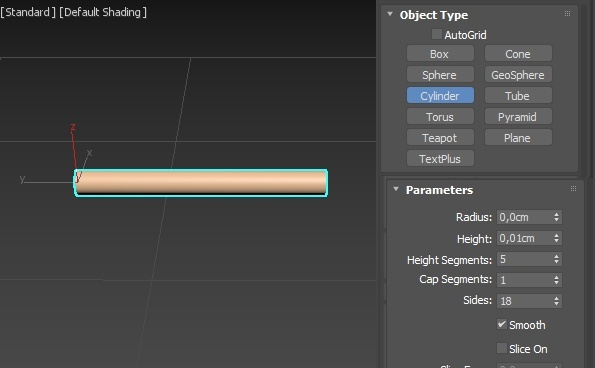
\includegraphics[width=0.8\textwidth]{image/modelovani.jpg} 
	\caption{Vytvoření cylinderu v 3ds Max.} 
	\label{fig:modelovani_cast1} 
\end{figure}



Tento postup budeme opakovat i pro tvorbu ostatních částí, na které zase použijeme cylinder, jen s jiným počtem stran. Strany se dají nastavit v parametrech. 

\begin{figure}[h!]
	\centering 
	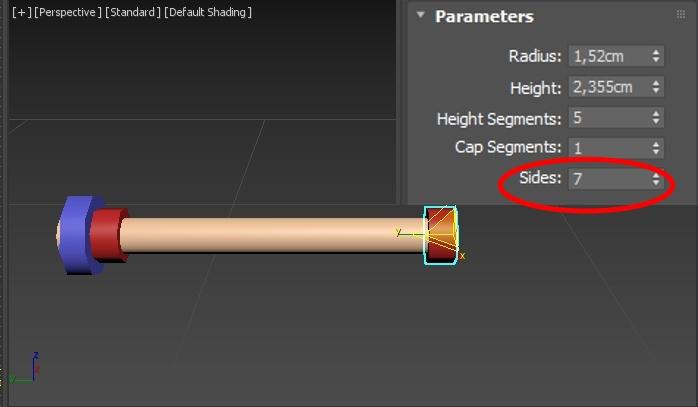
\includegraphics[width=0.5\textwidth]{image/modelovani2.jpg} 
	\caption{Tvorba dalších částí pístu.} 
	\label{fig:modelovani_cast2} 
\end{figure}


Pro obsáhlejší úpravu objektů můžeme použít Editable Poly, ve kterém se dá manipulovat s jednotlivými polygony, vertexy nebo hranami. Abychom je mohli vidět, musíme si zapnout Edged Faces.  

\begin{figure}[h!]
	\centering
	\subfloat{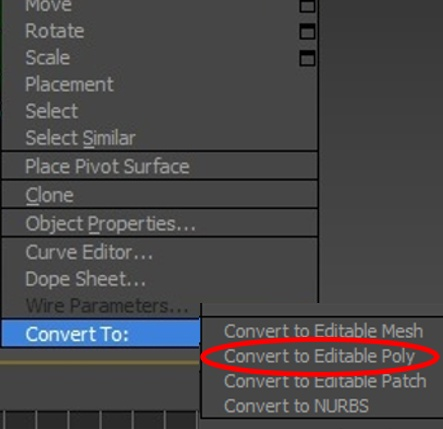
\includegraphics[width=7cm]{image/modelovani3.jpg}}
	\qquad
	\subfloat{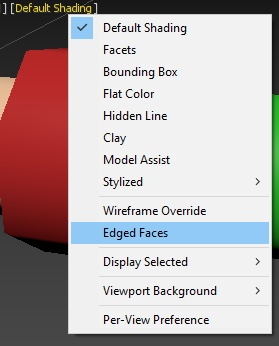
\includegraphics[width=7cm]{image/modelovani5.jpg}}
	\caption{Editable Poly a nastavení viditelnosti hran.}
	\label{fig:modelovani_cast3}
\end{figure}

\clearpage


Po vybrání všech hran objektu využijeme Connect, který nám spojí veškeré vybrané hrany. Na tyto hrany pak využijeme Extrude, který tyto hrany vytáhne podle našich požadavků.   

\begin{figure}[H]
	\centering
	\subfloat{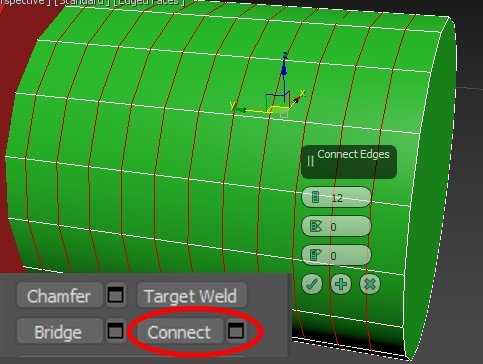
\includegraphics[width=7cm]{image/modelovani6.jpg}}
	\qquad
	\subfloat{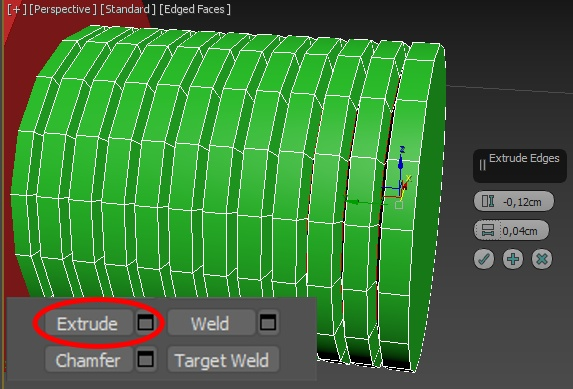
\includegraphics[width=7cm]{image/modelovani7.jpg}}
	\caption{Spojení a vytahnutí hran.}
	\label{fig:modelovani_cast4}
\end{figure}

Další část pístu také upravíme pomocí Connect. Poté pomocí Scale upravíme do potřebného tvaru. 

\begin{figure}[H]
	\centering
	\subfloat{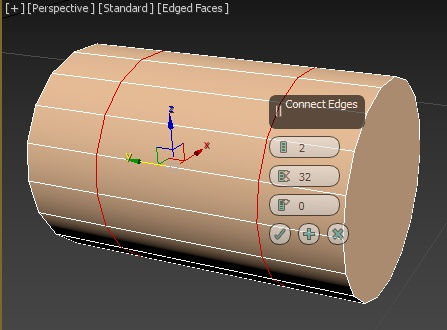
\includegraphics[width=7cm]{image/modelovani8.jpg}}
	\qquad
	\subfloat{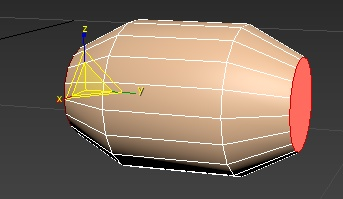
\includegraphics[width=7cm]{image/modelovani9.jpg}}
	\caption{Spojení hrany a úprava tvaru objektu pomocí Scale.}
	\label{fig:modelovani_cast5}
\end{figure}


Ze všech těchto objektů poté vytvoříme jeden jediný pomocí Attach. 

\begin{figure}[h!]
	\centering 
	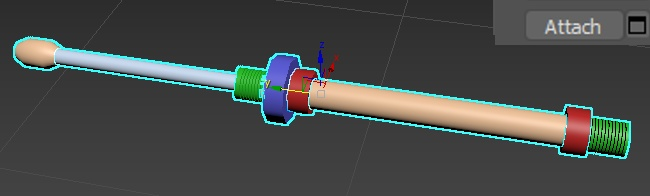
\includegraphics[width=0.8\textwidth]{image/modelovani10.jpg} 
	\caption{Spojení všech objektů do jednoho.} 
	\label{fig:modelovani_cast6} 
\end{figure}


\clearpage
\section {Nastavení materiálu objektů}
\label{material_objektu}
Po vymodelování objektu, je nutné mu přiřadit materiál. Všechny materiály jsem přiřazovala v 3ds Max, jelikož jsem v něm už s materiály pracovala.  Materiály se nastavují v Material Editor, kde je možné využití obrázku jako materiálu celého objektu nebo jen jeho části. Lze také použit pouhou barvu. Mimo vytvoření materiálu se v tomhle editoru dají také nastavit vlastnosti materiálu, jako je například průhlednost objektu nebo vyzařování světla z objektu.


\begin{figure}[h!]
	\centering
	\subfloat{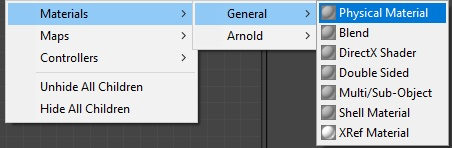
\includegraphics[width=7cm]{image/material.jpg}}
	\qquad
	\subfloat{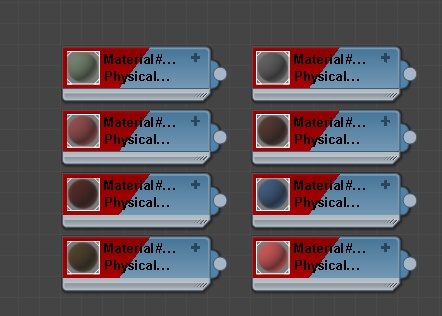
\includegraphics[width=7cm]{image/material1.jpg}}
	\caption{Ukázka  vytvoření nového materiálu a materiálů již vytvořených.}
	\label{fig:editor_materialu}
\end{figure}




\section {Importování do Unity}
\label{import_do_unity}
Všechny 3D objekty se dají do Unity importovat ve formátu .FBX, tento formát 3ds Max i~Blender podporuje. Takže žádný problém při importování souborů nenastává.

Při importování jednoduchých materiálu z 3ds Max také nevzniká ztráta materiálu, což znamená že jsem v Unity nemusela znovu nastavovat ani jeden materiál. 






\chapter{Mobilní aplikace v Unity}	

Svou celou aplikaci jsem vytvářela v Unity, což je multiplatformní herní engine, který nabízí spoustu balíčků, šablon a nástrojů pro vytváření nejrůznějších aplikací.  

	\section{Struktura projektu}
\label{sec:struktura_projektu}

		\begin{figure}[h!]
	\centering 
	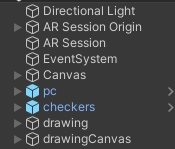
\includegraphics[width=0.4\textwidth]{image/hierarchy.jpg} 
	\caption{Ukázka hierarchie aktivní scény projektu.} 
	\label{fig:hierarchie} 
\end{figure}


	Projekt obsahuje několik podsložek. 
	3D objekty jsou uloženy ve složce Prefabs. Složka Scripts obsahuje veškeré mnou napsané skripty v C\#. Ve složce Animations jsou uložené animace a složka ReferenceImages obsahuje obrázky pro zobrazení 3D objektů. Unity si navíc vytváří i vlastní podsložky potřebné pro fungování celého projektu, také zde můžeme vidět stáhnuté balíčky, které mohou obsahovat skripty nebo objekty. Některé tyto balíčky se mohou stáhnout hned při vytvoření projektu, při použití šablony, nebo stáhnout později v Package Manager.
	
	
	
		\begin{figure}[h!]
		\centering 
		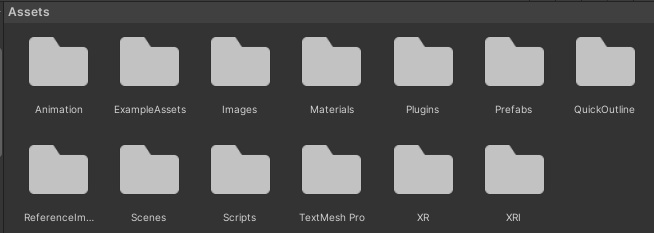
\includegraphics[width=0.8\textwidth]{image/assets.jpg} 
		\caption{Ukázka podsložek v projektu.} 
		\label{fig:podslozky} 
	\end{figure}
	
	
	
	\newpage
	
\section{Nastavení projektu}
\label{sec:nastaveni_projektu}
S pomocí šablony pro rozšířenou realitu, která obsahuje AR Foundation, což je framework určený pro vytváření rozšířené reality, je prvotní nastavení projektu jednoduché. AR Foundation obsahuje několik funkcí, které ulehčují práci s AR. Tato šablona také vlastnoručně přichystá základní nastavení celého projektu. 

K prvnímu spuštění celé aplikace je potřeba nastavit na jakou platformu chceme celý projekt směřovat. Protože jsem celou aplikaci testovala na Androidu, zvolila jsem si proto tuto platformu.

Hlavním aktérem celé aplikace je AR Session Origin, který obsahuje kameru a jsou na něj navázány nejrůznější skripty, které reagují na snímané prostředí. Skripty jsem použila jak vestavěné, tak i vlastní.

\begin{figure}[h!]
	\centering
	\subfloat{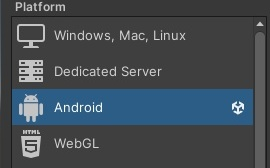
\includegraphics[width=7cm]{image/build.jpg}}
	\qquad
	\subfloat{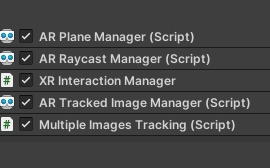
\includegraphics[width=7cm]{image/arorigincomponents.jpg}}
	\caption{Zvolení platformy a skripty připnuté k AR Session Originu.}
	\label{fig:nastaveni_unity}
\end{figure}


\newpage

\section {Sledování obrázků}
\label{sec:sledovani_obrazku}
 Sledování obrázku zajišťuje AR tracked image manager, který je součástí AR Foundation. Skládá se z manažeru a referenční knihovny (reference library). Součástí referenční knihovny jsou všechny obrázky, které chceme sledovat.
 
AR tracked image manager nás také za pomocí eventu trackedImagesChanged informuje o~každém přidaném, aktualizovaném nebo odstraněném obrázku. Nebo by alespoň měl; bohužel ale nikdy neoznámí odstranění obrázku, což způsobuje značné problémy. 

Naštěstí tento manažer také sleduje stavy jednotlivých obrázků. Správně by měl zobrazit jeden ze tří stavů (Tracking, Limited, None). I tady je tomu tak, že stav None nikdy nenastane a stav Limited nastane při jakémkoliv menším pohybu telefonu. 


\begin{lstlisting}[style=csh, caption={Ukázka kódu sledování obrázků.}]
	void OnTrackedImagesChanged(ARTrackedImagesChangedEventArgs eventArgs) {
		//added image
		foreach (var trackedImage in eventArgs.added) {
			UpdateARImage(trackedImage.referenceImage.name,trackedImage);
		}
		//updated image
		foreach (var trackedImage in eventArgs.updated) {
			//checking state of image
			if(trackedImage.trackingState != TrackingState.Tracking) {
				//hides menu if object is out of view
				if(state) {
					HideInteractible(trackedImage.referenceImage.name);	
				}
				else {
					//image is visible
					ShowInteractible(trackedImage.referenceImage.name);
					UpdateARImage(trackedImage.referenceImage.name,trackedImage);
				}
			}
		}
	}
\end{lstlisting}


\newpage

\section {Zobrazování 3D objektů}
\label{sec:zobrazovani_3d_objektu}
Zobrazování 3D objektů se odvíjí od sledovaného obrázku. Pokaždé, když se určitý obrázek přidá nebo aktualizuje, se podle něj objeví objekt se stejným jménem. 3D objekty dědí pozici obrázků. 

\section{Odstraňování 3D objektů}
\label{sec:odstraneni_3d_objektu}
Mým záměrem bylo odvíjet stavy objektů podle stavů sledovaných obrázků, ale kvůli špatné funkcionalitě jsem se rozhodla problém pro odstranění objektů vyřešit jinak, a to za pomocí Render.isVisible, který vrací, zda je určitý objekt zobrazen na jakékoliv kameře ve scéně. Pokud se objekt nenachází na jakékoliv kameře, objekt se odstraní. 

\begin{lstlisting}[style=csh, caption={Ukázka kódu zjišťování viditelnosti objektu.}]
 void Start() => m_Renderer = GetComponent<Renderer>();
void Update() {
	//sending state of object to different script
	MultipleImagesTracking.state = hide;
	if (m_Renderer.isVisible) hide = true;
	else {
		if (hide) {
			go.SetActive(false);
			hide = false;
		}
	}
}
}
\end{lstlisting}


\section{Canvas}
\label{sec:canvas}
Pro zobrazení grafických prvků se využívá plátno (canvas). Protože je Unity graficky založený engine, dá se většina jednoduchých operací naklikat bez použití vlastních skriptů. Pro účely své aplikace jsem na plátně vytvořila vlastní menu pro dodatečnou interakci s objekty. Zobrazení menu se řídí podle viditelnosti objektu. Canvas jsem také použila na vytvoření úvodního herního menu při prvním spuštění aplikace. 



\section{Funkce aplikace}
\label{funkce_aplikace}
Při spuštění aplikace se zobrazí úvodní menu, ve kterém jsou dvě možnosti „Play“ a „Cíl hry“. Při kliknutí na „Cíl hry“ se objeví krátký text, o čem vlastně aplikace je. 
Při volbě „Play“ se zapne kamera v telefonu. V pravém horním rohu se objeví ikonka počítače, na kterou se dá kliknout a zobrazit si tak hledané obrázky. Vlevo nahoře se nachází počet nalezených obrázků. 
Každý nalezený obrázek zobrazuje jiný 3D objekt, dokonce některé objekty nabízí i možnost interakce. 

\subsection{Dům}
Na sledovaném obrázku se zobrazí 3D model domu.  


\begin{figure}[H]
	\centering
	\subfloat{
\includegraphics[width=7cm]{image/houseImage.png}}
	\qquad
	\subfloat{
\includegraphics[width=8cm]{image/house.png}}
	\caption{Ukázka obrázku a modelu domu, který se na něm zobrazí.}
	\label{fig:house}
\end{figure}

\newpage

\subsection{Součástky mechatroniky}	
Jedná se o čtyři součástky používané v učebně mechatroniky: píst, kladka, pneumatický škrtič a modul s vypínači.
Jednotlivé součástky se dají procházet šipkami, které se objeví při zobrazení prvního objektu. Píst a kladka mají vlastní animaci, která ukazuje, jak se pohybují. 


\begin{figure}[H]
	\centering 
	
\includegraphics[width=0.25\textwidth]{image/mechatronika.png} 
	\caption{Obrázek, na kterém se zobrazí modely součástky.} 
	\label{fig:mechatronika_obrazek} 
\end{figure}


\begin{figure}[H]
	\centering
	\subfloat{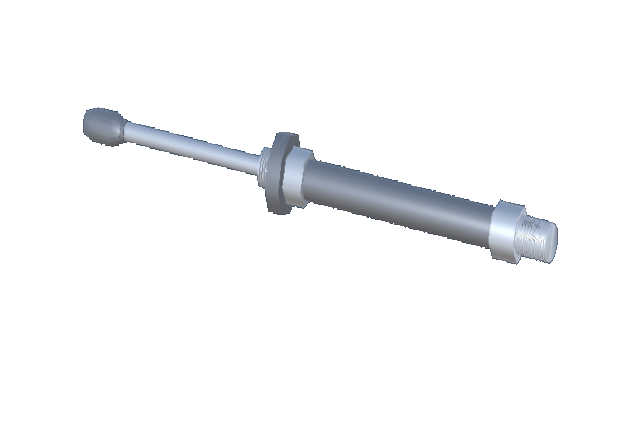
\includegraphics[width=7cm]{image/pist.png}}
	\qquad
	\subfloat{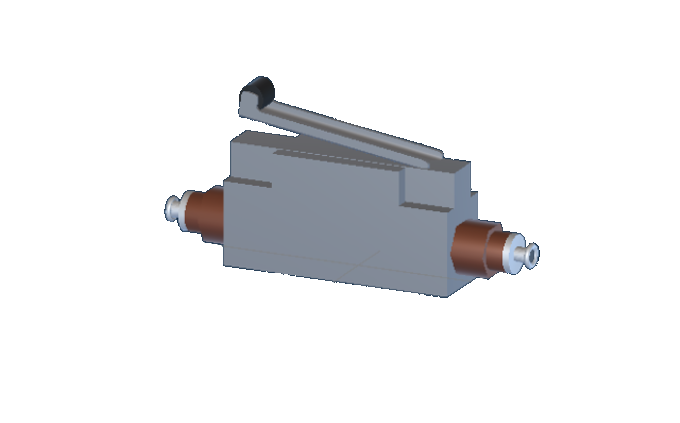
\includegraphics[width=7cm]{image/kladka.png}}
	\caption{3D modely pístu a kladky.}
	\label{fig:soucastky}
\end{figure}

\begin{figure}[H]
	\centering
	\subfloat{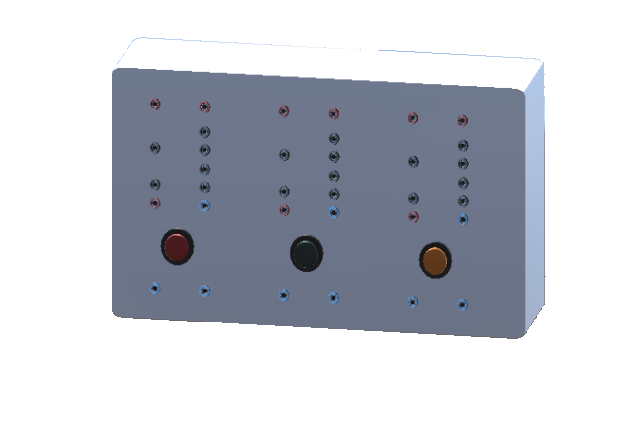
\includegraphics[width=7cm]{image/modul.png}}
	\qquad
	\subfloat{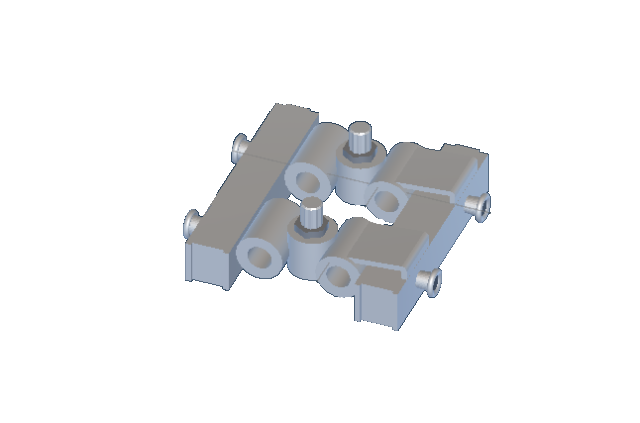
\includegraphics[width=7cm]{image/skrtic.png}}
	\caption{3D modely modulu s vypínači a pneumatického škrtiče.}
	\label{fig:soucastky2}
\end{figure}

\newpage

\subsection{Počítač}	
Jeden z obrázků zobrazuje model počítače, kterému jde odstranit kryt. Když se kryt odstraní, je možné klikat na některé počítačové komponenty, které po kliknutí zobrazí menu se zvětšeným zvoleným komponentem, který se začne otáčet. Vedle něj je krátký popis o úloze komponentu v počítači.

K označení komponentů napomáhá balíček QuickOutline, který jsem si stáhla k mému projektu. Celý tento balíček vytváří obrysy pro objekty. Využití je velmi jednoduché. Připneme k~objektu, kterému chceme přidat obrys, popřípadě můžeme zobrazení obrysu detailněji nastavit v editoru. 

Interakce s celým počítačem je zařízena pomocí XR Interaction Toolkit, který zprostředkovává lepší interakci s objekty. Součástí je Interactive Manager, ve kterém se dají nastavit různé možnosti interakce. Pro své potřeby jsem použila pouze funkci pro vybírání objektů. Při kliknutí na objekt se spustí skript pro zobrazení menu komponentu.


\begin{figure}[!h]
	\centering 
	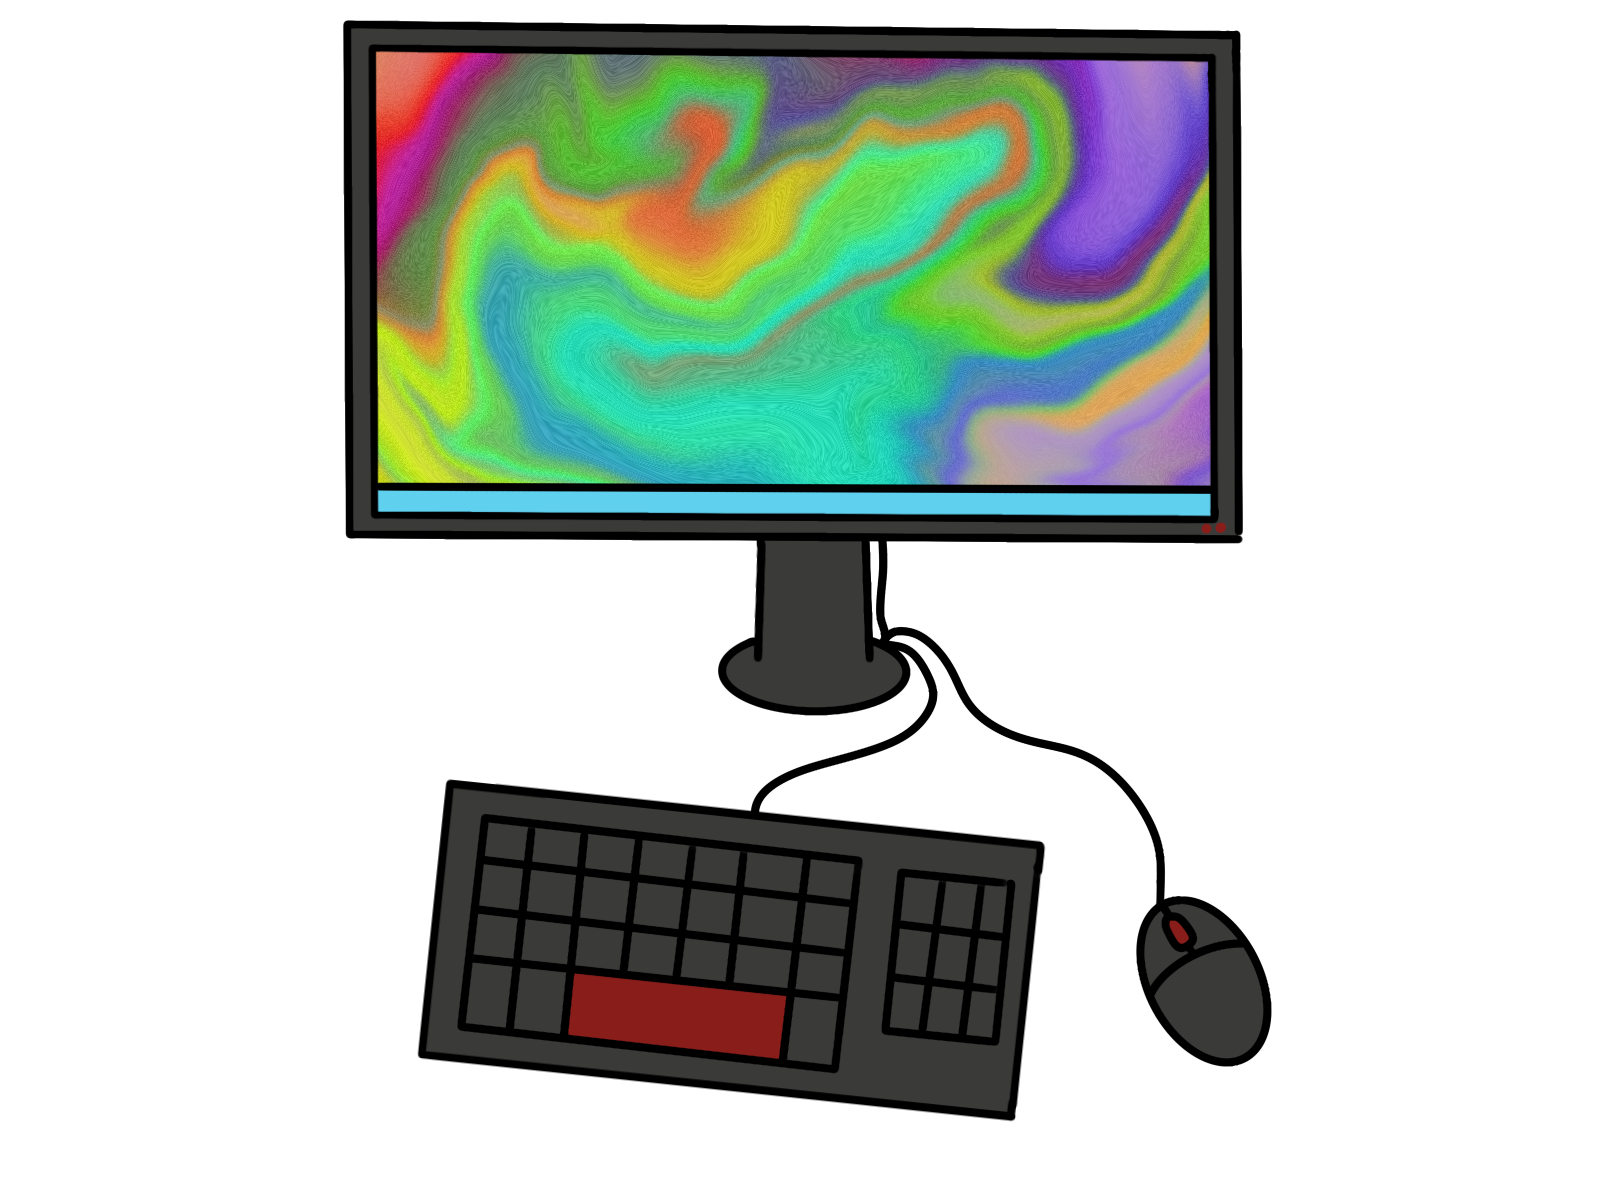
\includegraphics[width=0.3\textwidth]{image/pcImage.png} 
	\caption{Ukázka obrázku, na kterém se zobrazí model počítače.} 
	\label{fig:pc_obrazek} 
\end{figure}

\begin{figure}[H]
	\centering 
	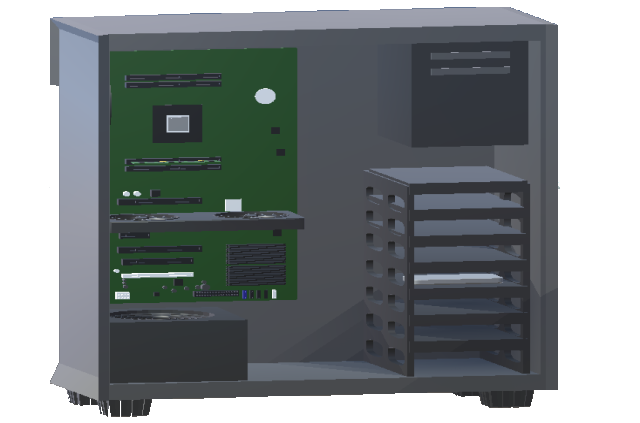
\includegraphics[width=0.6\textwidth]{image/pc.png} 
	\caption{3D objekt počítače s označenými komponenty zahrnující: paměti RAM, základní desku, procesor, grafickou kartu, napájecí zdroj počítače a SSD disk.} 
	\label{fig:pc} 
\end{figure}


\begin{figure}[H]
	\centering
	\subfloat{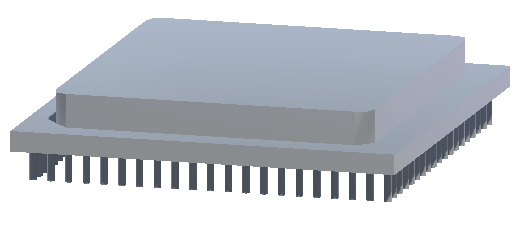
\includegraphics[width=7cm]{image/cpu.png}}
	\qquad
	\subfloat{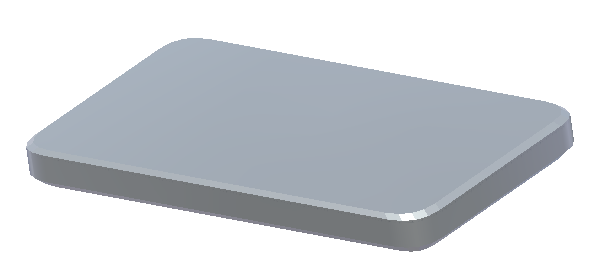
\includegraphics[width=7cm]{image/ssd.png}}
	\caption{3D modely procesoru a SSD disku.}
	\label{fig:components}
\end{figure}

\begin{figure}[H]
	\centering
	\subfloat{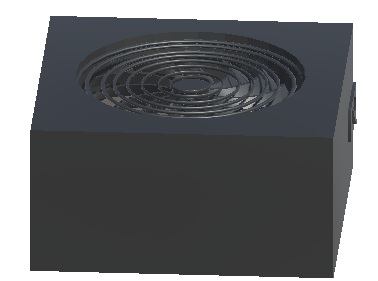
\includegraphics[width=7cm]{image/psu.png}}
	\qquad
	\subfloat{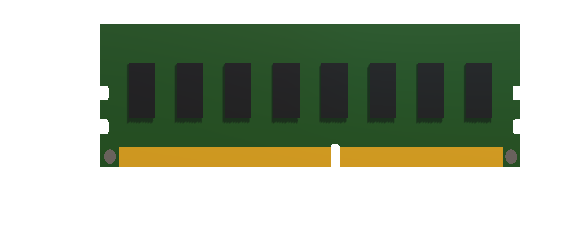
\includegraphics[width=7cm]{image/ram.png}}
	\caption{3D modely napájecího zdroje počítače a paměti RAM.}
	\label{fig:components2}
\end{figure}

\begin{figure}[H]
	\centering 
	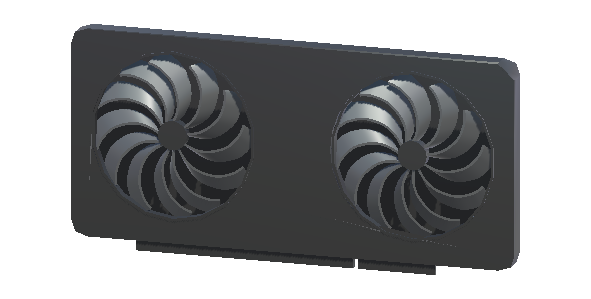
\includegraphics[width=0.6\textwidth]{image/gpu.png} 
	\caption{3D objekt grafické karty.} 
	\label{fig:components3} 
\end{figure}

\newpage

\subsection{Dáma}	
Umožňuje hrát dámu při nalezení obrázku figurky pěšce, kromě hrací plochy dámy se také objevuje tlačítko „Restart“ umožňující restartovat rozehranou hru, „Pravidla“, které vysvětlují základní princip hry, a text, který oznamuje, který hráč je na řadě. Dáma je jen zjednodušená, což znamená, že neřeší povinné skákání ani změnění kamene na dámu při doskákání na druhou stranu šachovnice. První tah vždy začíná červený kámen.  

Dáma také využívá Interactive Manager, který spouští skripty ovládající celou hru. Při kliknutí na kámen se uloží pozice, na které kámen leží. Podle ní se poté určují další možné tahy kamene. 


\begin{figure}[H]
	\centering
	\subfloat{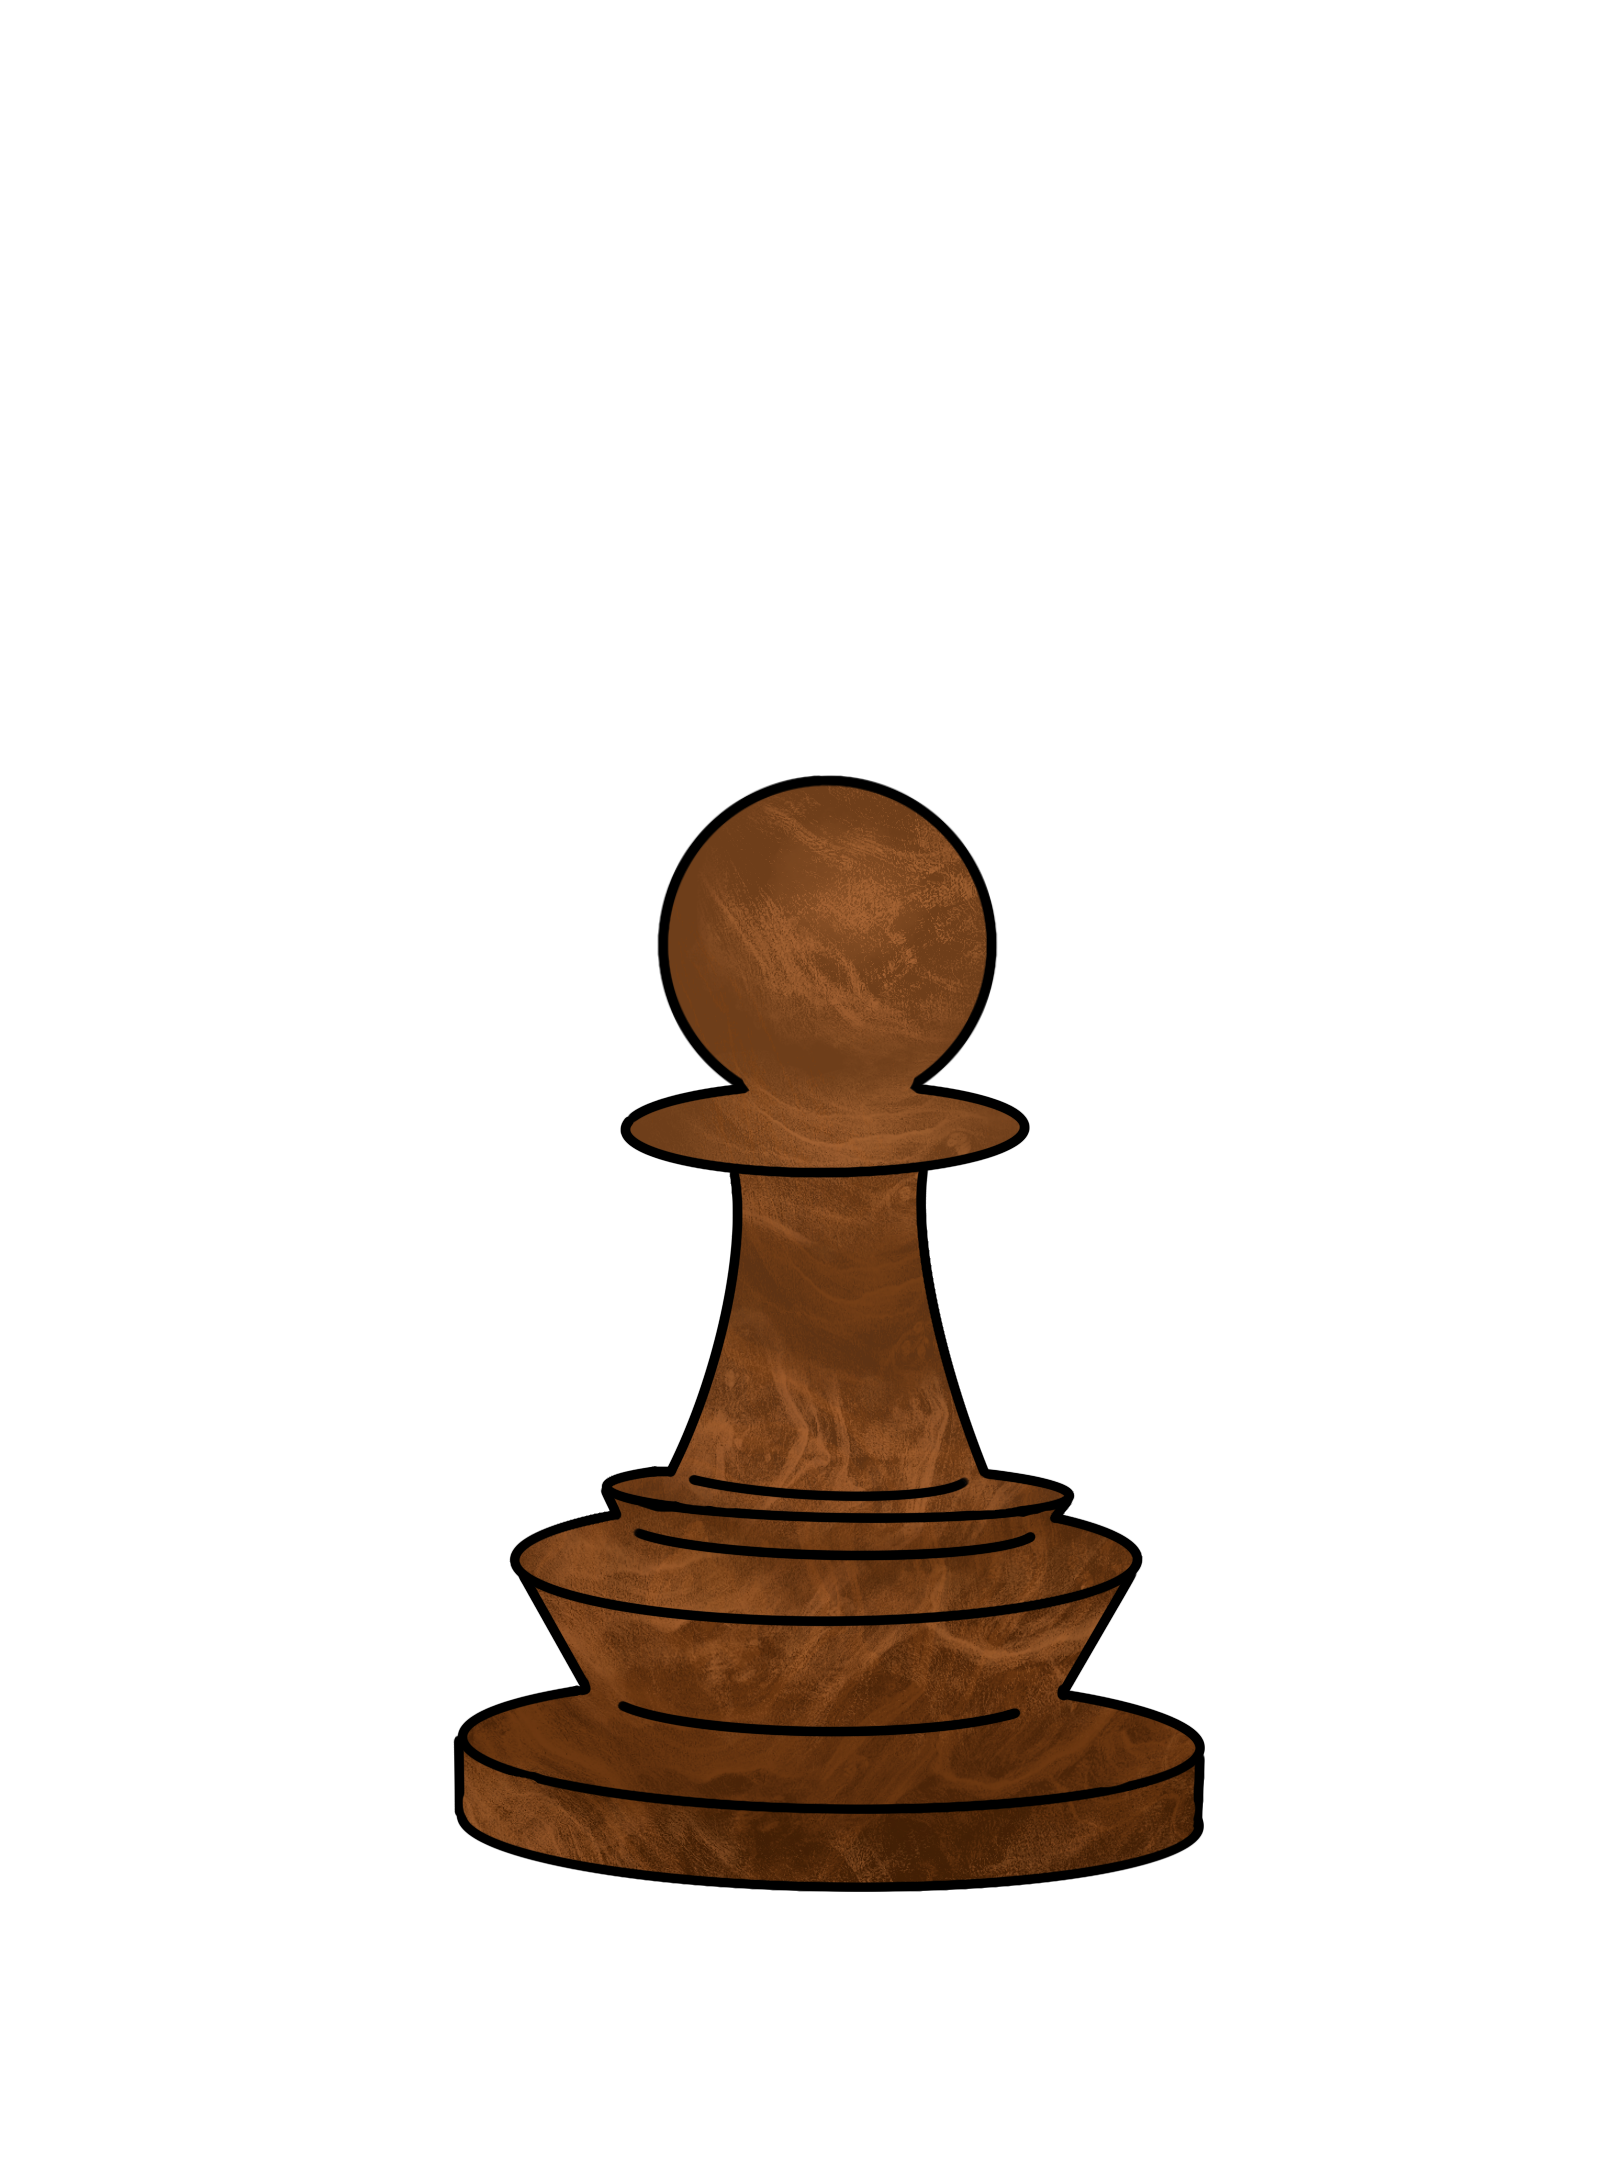
\includegraphics[width=7cm]{image/checkersImage.png}}
	\qquad
	\subfloat{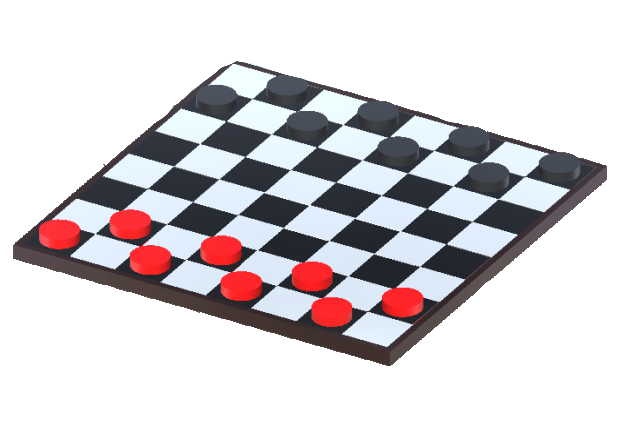
\includegraphics[width=7cm]{image/checkers.png}}
	\caption{Ukázka obrázku a modelu dámy, který se na něm zobrazí.}
	\label{fig:checkers}
\end{figure}

\newpage

\subsection{Kreslení}
Při zobrazení objektu se odemkne možnost kreslení, rovněž se zobrazí menu s tlačítkem „Vymazání“, které smaže celý nakreslený obsah, a výběrem kreslící barvy, který obsahuje zelenou, červenou, modrou a černou. Na tuto část projektu jsem využila tutoriál: How to Create AR Draw/Doodling in Unity3D \cite{ardrawing}.

\begin{figure}[H]
	\centering
	\subfloat{
\includegraphics[width=6cm]{image/drawingCanvas.png}}
	\qquad
	\subfloat{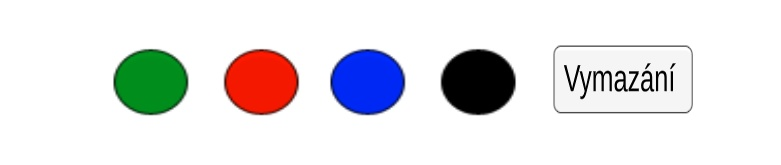
\includegraphics[width=6cm]{image/drawing.jpg}}
	\caption{Ukázka obrázku pro spuštění kreslení a výběru barvy kreslení.}
	\label{fig:drawing}
\end{figure}



	
\chapter*{Závěr}
\addcontentsline{toc}{chapter}{Závěr}
Cílem projektu bylo vytvoření aplikace s rozšířenou realitou. Tento cíl se mi povedlo uskutečnit. Výsledkem mé práce je aplikace, která obsahuje úvodní menu a 3D objekty, které se zobrazují při nalezení obrázků. Některé tyto 3D objekty nabízí možnost interakce jako například možnost hraní dámy, kreslení či interakce s vymodelovaným počítačem. 
 
 Také jsem se více seznámila s~problematikou rozšířené reality a pracování v Unity. 
 
 Kdybych práci vypracovávala znovu, nejspíše bych použila jiný framework než AR Foundation, a tak bych snad obešla již zmíněný problém se sledováním obrázků. 
 
 Jedno z možných vylepšení do budoucna je tvorba více objektů s jinými možnostmi interakce.

Odkaz na projekt: \url{https://github.com/MajkeltCZe/zaverecny-projekt}


%% Seznam použitých informačních zdrojů
\renewcommand\bibname{Seznam použitých informačních zdrojů}
\begin{thebibliography}{99}
\addcontentsline{toc}{chapter}{Seznam použitých informačních zdrojů}
\bibitem{ARImageTracking} \textit{AR Foundation Improved Image Tracking - Multiple Objects/Images - Unity Augmented Reality/AR} [online]. YouTube, 5.4.2020 [cit. 2023-12-18]. Dostupné z: \url{https://www.youtube.com/watch?v=I9j3MD7gS5Y}

\bibitem{animations} \textit{Create UI ANIMATIONS without CODING! - Unity UI tutorial} [online]. YouTube, 24.3.2021 [cit. 2023-12-18]. Dostupné z: \url{https://www.youtube.com/watch?v=br9YzpiBeIw}	

\bibitem{arvyuziti}\textit{Hospodářské noviny: Pět oblastí, kde můžete nejlépe využít rozšířenou realitu} [online]. [cit. 2023-12-17]. Dostupné z: \url{https://hn.cz/c1-66644350-pet-oblasti-kde-muzete-nejlepe-vyuzit-rozsirenou-realitu}

\bibitem{variables} \textit{How to get a variable from another script in Unity (the right way)} [online]. YouTube, 6.7.2022 [cit. 2023-12-18]. Dostupné z: \url{https://www.youtube.com/watch?v=2pCkInvkwZ0}

\bibitem{ardrawing}\textit{Medium: 
How to Create AR Draw/Doodling in Unity3D} [online]. [cit. 2023-12-17]. Dostupné z: \url{https://medium.com/antaeus-ar/how-to-create-ar-draw-doodling-in-unity3d-ar-foundation-233b0e0f921e}

\bibitem{onirix}\textit{Onirix: What Are The Different Types of Augmented Reality?} [online]. [cit. 2023-12-17]. Dostupné z: \url{https://www.onirix.com/learn-about-ar/types-of-augmented-reality}

\bibitem{arraysListDictionaries}\textit{Packt Hub: How to use arrays, lists, and dictionaries in Unity for 3D game development} [online]. [cit. 2023-12-17]. Dostupné z: \url{https://hub.packtpub.com/arrays-lists-dictionaries-unity-3d-game-development}

\bibitem{gamePreviewOnMobile} \textit{Quickly preview your game on Android device | Unity tutorial} [online]. YouTube, 25.6.2021 [cit. 2023-12-18]. Dostupné z: \url{https://www.youtube.com/watch?v=iCXwaehzRFQ}

\bibitem{quickOutline}\textit{Quick Outline: Particles/Effects} [online]. [cit. 2023-12-17]. Dostupné z: \url{https://assetstore.unity.com/packages/tools/particles-effects/quick-outline-115488}

\bibitem{uiMouseOver} \textit{Quick Tip: Test Mouse over UI | Unity Tutorial} [online]. YouTube, 24.5.2018 [cit. 2023-12-18]. Dostupné z: \url{https://www.youtube.com/watch?v=ptmum1FXiLE}

\bibitem{unityRichText}\textit{Rich Text: Unity UI: 1.0.0} [online]. [cit. 2023-12-17]. Dostupné z: \url{https://docs.unity3d.com/Packages/com.unity.ugui@1.0/manual/StyledText.html}

\bibitem{artypes}\textit{Shopify: 5 Types of AR and How They Improve Online Shopping} [online]. [cit. 2023-12-17]. Dostupné z: \url{https://www.shopify.com/blog/types-of-ar}	

\bibitem{menu} \textit{START MENU in Unity} [online]. YouTube, 29.11.2017 [cit. 2023-12-18]. Dostupné z: \url{https://www.youtube.com/watch?v=zc8ac_qUXQY}

\bibitem{unityAssetStore}\textit{Unity Asset Store: The Best Assets for Game Making} [Online]. [cit. 2023-12-17]. Dostupné z: \url{https://assetstore.unity.com}

\bibitem{imagetracking}\textit{Unity: Ar tracked image manager: AR Foundation: 4.0.12} [online]. [cit. 2-17]. Dostupné z: \url{https://docs.unity3d.com/Packages/com.unity.xr.arfoundation@4.0/manual/tracked-image-manager.html}

\bibitem{unityExecution}\textit{Unity: Order of execution for event functions} [online]. [cit. 2023-12-17]. Dostupné z: \url{https://docs.unity3d.com/Manual/ExecutionOrder.html}

\bibitem{unityReference}\textit{Unity: Welcome to the Unity Scripting Reference!} [online]. [cit. 2023-12-17]. Dostupné z: \url{https://docs.unity3d.com/ScriptReference/}

\bibitem{instantiatingGameObjects} \textit{Unity3d with AR Foundation - How To Instantiate A Game Object Per Tracked Image?} [online]. YouTube, 24.9.2019 [cit. 2023-12-18]. Dostupné z: \url{https://www.youtube.com/watch?v=iM0ghkvsRos}

\bibitem{uvoddoAR}\textit{Úvod do tématu: Rozšířená realita (AR) ve vzdělávání: O2 Chytrá škola} [online]. [cit. 2023-12-17]. Dostupné z: \url{https://vyuka.o2chytraskola.cz/clanek/54/rozsirena-realita-ar-ve-vzdelavani}

\bibitem{xrinteractionToolkit}\textit{XR Interaction Toolkit: XR Interaction Toolkit: 0.9.4-preview} [online]. [cit. 2023-12-17]. Dostupné z: \url{https://docs.unity3d.com/tages/com.unity.xr.interaction.toolkit@0.9/manual/index.html}



\end{thebibliography}

%% obrázky 
\listoffigures



\end{document}